\section{PS0: Hello SFML}\label{sec:ps0}
\graphicspath{{ps0}}
\subsection{Discussion:}\label{sec:ps0:disc}
 
       
 
    The first project of CompIV 22 is \textbf{Hello World with SFML}. In this assignment, At first we set up our environment by installing the SFML library. We also check for the newest version of the C++. Thereby, We test the given code and check whether it is working or not. At the last part of the assignment we include and image and use the sprite property of the SFML to move the image using the Keys of the Keyboard. The output is in\textbf{ Figure: \ref{fig:ps0}} 

\subsection{Key algorithms, Data structures and OO Designs used in this Assignment:}\label{sec:ps0:kdo}

    This assignment did not require any of the key algorithm, Data structures and OO Designs, as the project it self is basic project with the code provided and we just had to add SFML sprite and few Keyboard events to complete the project.
    So, There is no use of the Algorithms and Data Structures.


\subsection{Images used:}\label{sec:ps0:img}
\begin{figure}[h]
    \centering
    
\includegraphics[width=0.25\textwidth]{ps0/sprite.png}
    \caption{Sprite Image}
    \label{fig:mesh1}
\end{figure}

\subsection{What I accomplished :}\label{sec:ps0:accomplish}

I accomplished to move the Sprite image using Keyboard keys as well as with the Mouse click.

\subsection{What I already knew :}\label{sec:ps0:knew}

I was aware of how to move the image using keyboard keys and also mouse pointer events as I already learnt Javascript. So, It was much easy to do. I know SFML is different than JavaScript but the concept of it is similar to me.

\subsection{What I learned :}\label{sec:ps0:learn}

I learned to use SFML for the first time and also how to add events and manipulate them in the SFML field.
Overall, It was fun to do this assignment, as everything for me in this assignment was new an amazing.

\subsection{Challenges :}\label{sec:ps0:challenges}

Setting up the SFML environment was challenging to me. Also learning much about the SFML functions.
\subsection{Acknowledgements:}
\begin{itemize}
    \item \url{https://www.sfml-dev.org/tutorials/2.5/}
    \item \url{https://youtu.be/axIgxBQVBg0}
\end{itemize}
\newpage

\subsection{Codebase}\label{sec:ps0:code}

\colorbox{pink}{\textbf{Makefile:}} \newline \textbf{This Makefile was provided in portal.}
\lstinputlisting[language=Make]{ps0/Makefile} 

\colorbox{pink}{\textbf{main.cpp:}} \newline \textbf{The main file where the code runs and provides the valid output as shown in figure 2.}
\lstinputlisting{ps0/main.cpp}


\subsection{Output:}\label{sec:ps0:output}
\begin{figure}[h]
    \centering
    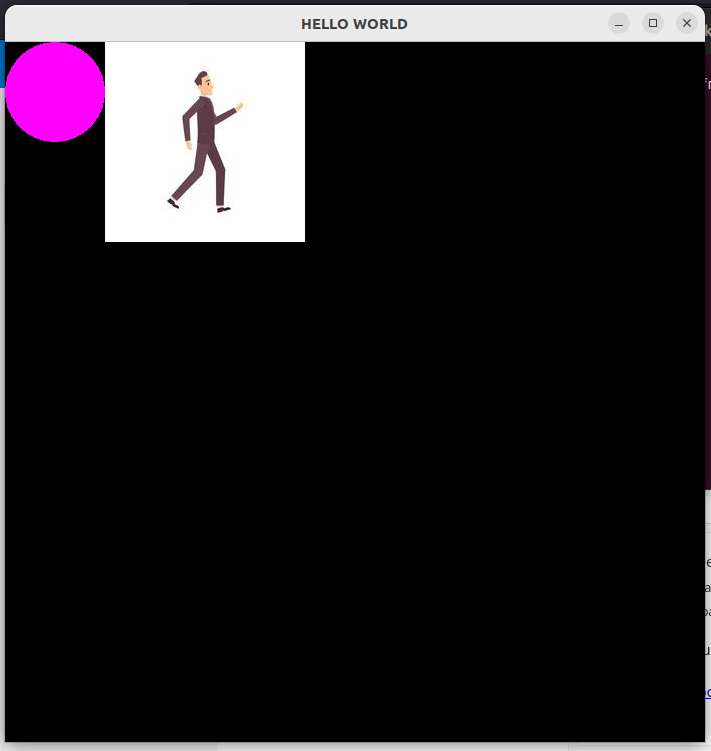
\includegraphics[width=0.5\textwidth]{ps0/Screenshot.png}
    \caption{Output of PS0 Assignment}
    \label{fig:ps0}
\end{figure}



\newpage
